\chapter{多国家定量脑电谱常模演化曲面研究}
\section{研究背景}
前面几章中参考选择和谱质量筛选准则研究为进行大样本定量脑电分析奠定质量基础。定量脑电是基于静息态脑电谱常模特征的诊断方法说明构建谱常模是定量脑电分析的关键内容,其作为一种无创工具已在神经系统疾病和健康人群脑功能研究中广泛应用\citing{cohen2017does}。功率谱总结出脑电活动的线性稳态特征,与不同行为状态有关。静息态脑电谱含有四个基本节律频带\citing{babiloni2018s178}:慢波高幅与睡眠有关的$\delta$节律(0.5-3.5Hz),更快波且幅度增加与困倦状态相关的$\theta$节律(4-7Hz),与放松和闭眼状态有关的$\alpha$节律(8-12Hz)以及清
醒警觉状态下的$\beta$节律(13-30Hz)。论文\citing{john1988neurometrics,buzsaki2006rhythms}发现$\alpha$节律谱峰与各种认知功能和精神疾病状态有关。功率谱是研究大脑信息处理和状态\citing{babiloni2004human,Li2019eeg}机制的常用手段。

谱特征与正常值的偏差可通过正常脑电数据库关于年龄因素做z变换调整后的谱特征均值和标准偏差来判定,z变换得到的曲线或曲面称为谱常模演化公式或曲面\citing{john1980developmental}。原始脑电主要特征的描述参数可弥补视觉定性分析的不足。基于宽带谱与单个频率点窄带谱的参数估计略有不同。描述参数通过z变换得到尺度调整且高度依赖于年龄。正常数据库中谱描述参数的z分数标准化\citing{glantz1990primer}变换如下:\(z=\frac{x-\mu}{\sigma}\),这里$x$是任何谱相关的参数,$\mu$和$\sigma$分别是正常人群该谱参数的均值和标准偏差。引入年龄和其他协变量能增加模型特异性和敏感性。该观点被论文\citing{john1980developmental}证明,随后得到研究\citing{matouvsek1973automatic,john1977neurometrics,alvarez1987eeg,amador1989structure}等的验证。因此,谱常模通常是宽带谱特征关于年龄的回归函数。

研究\citing{alvarez1987eeg}用脑电常模演化公式比较古巴和美国孩子,其中的演化公式模型源自美国人群分析\citing{john1980developmental},E R John等认为常模相对独立于社会文化等因素且应存在跨文化间的可行性,但仅采用了宽带谱参数分析。Koenig的论文\citing{koenig2002millisecond}用多国家496例脑电数据在毫秒时间分辨率比较微状态空间模式和特征,肯定脑电特征与年龄的强烈依赖关系。但Koenig并没进行频谱分析,其研究结果与脑电频域演化特征并不相关。本章是首个构建多国家脑电
数据频谱常模的研究。脑电常模估计中,古巴研究团队的主要发现之一是宽带$\delta$、$\theta$、$\alpha$、$\beta$谱与窄带谱存在不同。古巴研究团队对定量脑电模型和脑电常模的研究描述在论文\citing{hernandez-gonzalez_multimodal_2011}中,文中介绍古巴人类脑影像计划分为19世纪90年代和2004-2006年两个阶段,他们探究高分辨率谱模型作为宽带谱模型的替代选择。研究\citing{szava1994high}发现高分辨率下的脑电常模演化曲面能避免宽带谱常模在频域和空间上的混叠。 接收操作特征(Receiver Operating Characteristic, ROC)曲线分析证明高分辨率谱方法有更高的诊断准确率。 另外,论文\citing{amador1990spatiotemporal}引入回归公式来计算演化曲面,描述了健康人群$\log$变换后的功率谱均值与标准偏差关于频率和年龄的分布。构建常模曲面需要计算所有电极的功率谱以及每个频率点关于年龄的z分布。

某个孤立地区的谱常模已不能满足当前建立国际大样本脑电数据库进行定量分析的需求,脑电谱常模如何受到国家和个体的影响尚不清楚。神经科学的主要问题之一是从大量健康人群中获取影像数据并推断不同认知和情绪状态的潜在机制。常模可为识别大脑病理相关的状态提供有用信息,提高干预神经老化、治疗精神紊乱方法的有效性。但用神经影像数据获取常模相当困难,如难以对不同磁共振扫描机复杂的数据记录过程实现统一,磁共振不同梯度间的比较也不可靠,更不用说最终估计常模。与此类似,脑电要处理放大器和记录系统间的差异及参考电极问题\citing{hu_how_2018}等。国际脑影像计划正努力开展跟踪研究收集数以千计的被试,虽然目前人类脑连接计划\citing{van2013wu}以功能磁共振和脑磁图为主,但很可能会引入脑电。这里用古巴人脑计划\citing{hernandez-gonzalez_multimodal_2011}中的脑电数据验证建立多国家谱常模的假设。

本章的研究问题是脑电窄带特征个体间差异较大,能否建立不依赖于国家和个体因素的常模;能否通过新方法建立大样本国际通用谱常模。研究\citing{john1977neurometrics}首次表明脑电宽带谱特征不受国家、民族与采集设备的影响,但该结果尚未在窄带脑电谱特征中得到验证。本章假设健康被试的脑电常模特征关于国家因素没有显著差异,首次报道大样本多国家脑电谱常模演化曲面。
采用平均参考和专家甄选,分析来自瑞士、美国和古巴的535例被试脑电数据,构建多国家谱常模演化曲面。通过线性混合效应模型分析所有样本$\log$尺度脑电功率谱与年龄、频率、国家和个体等自变量的关系,发现被试的出生国家对谱特征没有显著影响且与其它自变量没有交互关系,然而谱特征与年龄和频率高度相关。为准确估计谱常模演化曲面,对谱曲线在年龄和频率维度上进行非参数回归得到谱常模演化曲面发现:1.慢波节律$\delta$、$\theta$在被试年龄较小时占更大比例,随着年龄增加逐渐减弱直至随后消失;2.$\alpha$节律在年纪较小时不存在,随着神经发育逐渐出现在枕顶叶且该节律的中心频率逐渐变高。该结果是神经发育和成熟
脑电谱特征的常模表达式,是首个使用多国家脑电数据构建定量脑电谱演化曲面的研究。
\section{研究方法}
\subsection{数据样本}
来自三个国家的535例均按照10-20电极放置系统采集的静息态脑电数据:
\begin{description}
\item[250例] 古巴人类脑影像计划中古巴神经科学中心分别在19世纪90年代采集的162例数据和2004-2006年间采集的88例数据。
\item[43例] 瑞士伯恩临床精神医院大学采集的43例数据。
\item[242例] 美国纽约大学医学院脑研究实验室的242例数据。
\end{description}
论文\citing{john1977neurometrics,alvarez1987eeg,koenig2002millisecond,hernandez-gonzalez_multimodal_2011}描述了健康被试的遴选标准,所有被试在接近同等条件下采集数据,
记录脑电时的被试年龄范围是5.35-97岁。样本的年龄分布如图\ref{6:age}所示,图\ref{6:age}A说明多国家数据样本包含更多儿童和青少年、适量中年人和较少65岁以上的老年人。图\ref{6:age}B说明古巴19世纪90年代收集的数据覆盖5.35-97岁接近整个生命周期,2004年左右收集的数据主要覆盖17.5-47.22岁的成年人,瑞士和美国的样本年龄分别是10.17-16.25岁和6.02-25.93岁。
\begin{figure}[!ht]
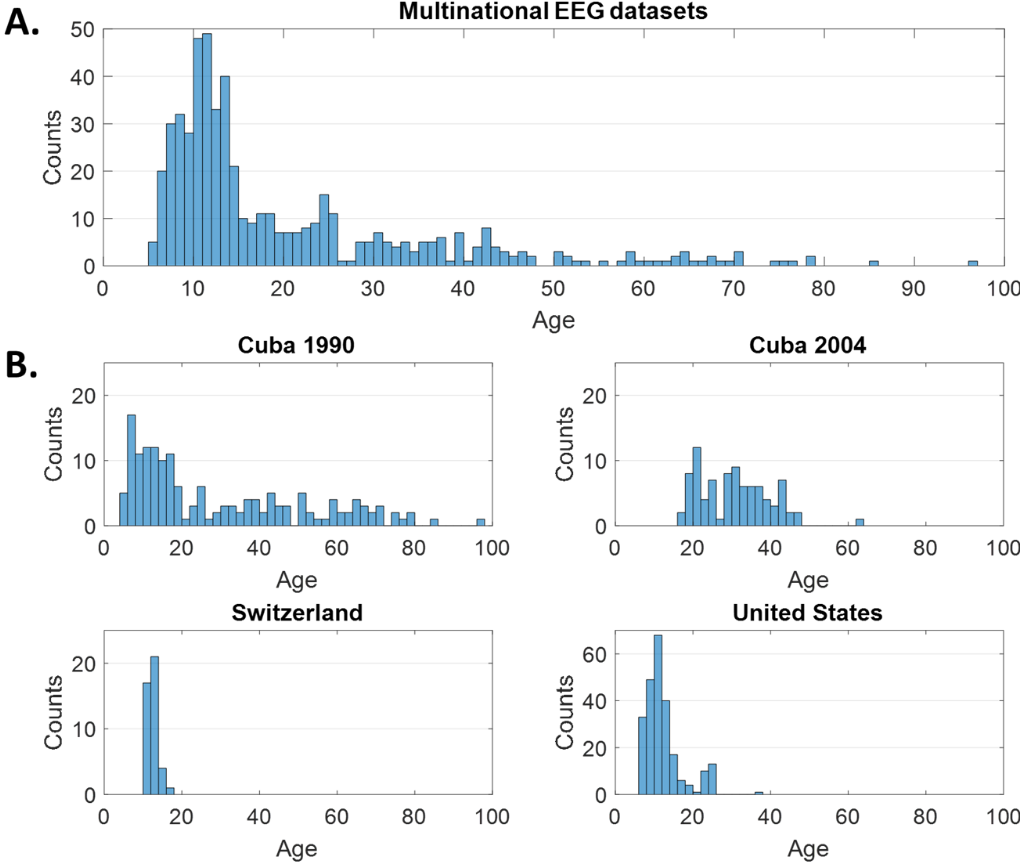
\includegraphics[width=15cm]{pic/Norm/figure1.png}
\caption{多国家脑电数据中覆盖生命周期的年龄分布直方图。 A.所有数据汇总视图,B.每个国家数据视图。}
\label{6:age}
\end{figure}

古巴被试是从哈瓦那市约11万人口中随机选出的603个被试\citing{hernandez-gonzalez_multimodal_2011}。闭眼静息态数字脑电是所有活跃电极同时参考到连接耳\citing{hu_unified_2018,hu_statistics_2019}采集得到,电极放置系统按照国际10-20电极放置系统(Fp1、Fp2、F3、F4、C3、C4、P3、P4、O1、O2、F7、F8、T3、T4、T5、T6、Fz、Cz和Pz)。 电极分布如图\ref{6:ele}所示,参考模态如图\ref{6:amp}B所示。所有被试的静息态脑电都是在安静且灯光昏暗并进行温控的房间内记录。记录过程中,被试坐在舒适的半斜臂椅上休息。古巴脑电采集的两个阶段使用相同类型如图\ref{6:amp}A所示的MEDICID 03 Neurometric(NEURONIC S. A.)放大器系统,但在2004年左右采集时比19世纪90年代用了更多电极。瑞士脑电数据记录时采用Nihon-Kohen标准脑电设备,具有与古巴脑电采集
设备相似的参数和性能。美国纽约大学脑研究实验室设计了如图\ref{6:amp}B所示的数字脑电数据采集分析系统(DEDAAS)\citing{thatcher1977functional}。所有数据采样率均为200Hz,每个被试可用数据
为最短60s的连续无明显噪声片段。所有被试均签有知情同意书并经对应研究中心的伦理道德委员会批准。
\bigskip
\begin{figure}[!h]
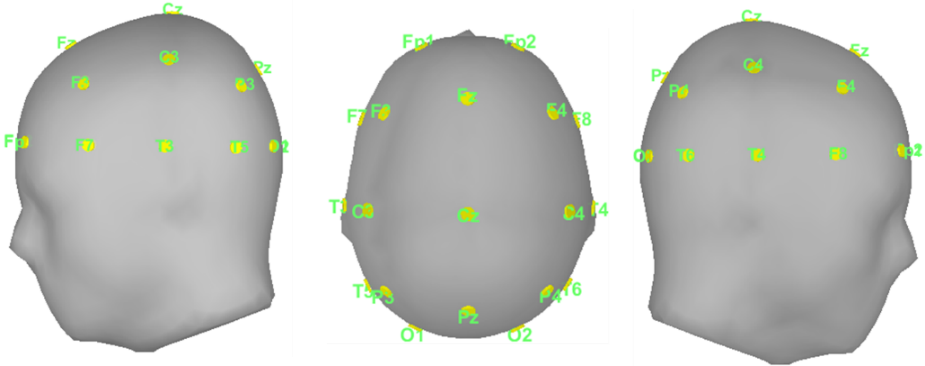
\includegraphics[width=13cm]{pic/Norm/figure2.png}
\caption{与ICBM152\citing{tadel2011brainstorm}模板配准的国际10-20电极放置系统。}
\label{6:ele}
\end{figure}

\begin{figure}[!h]
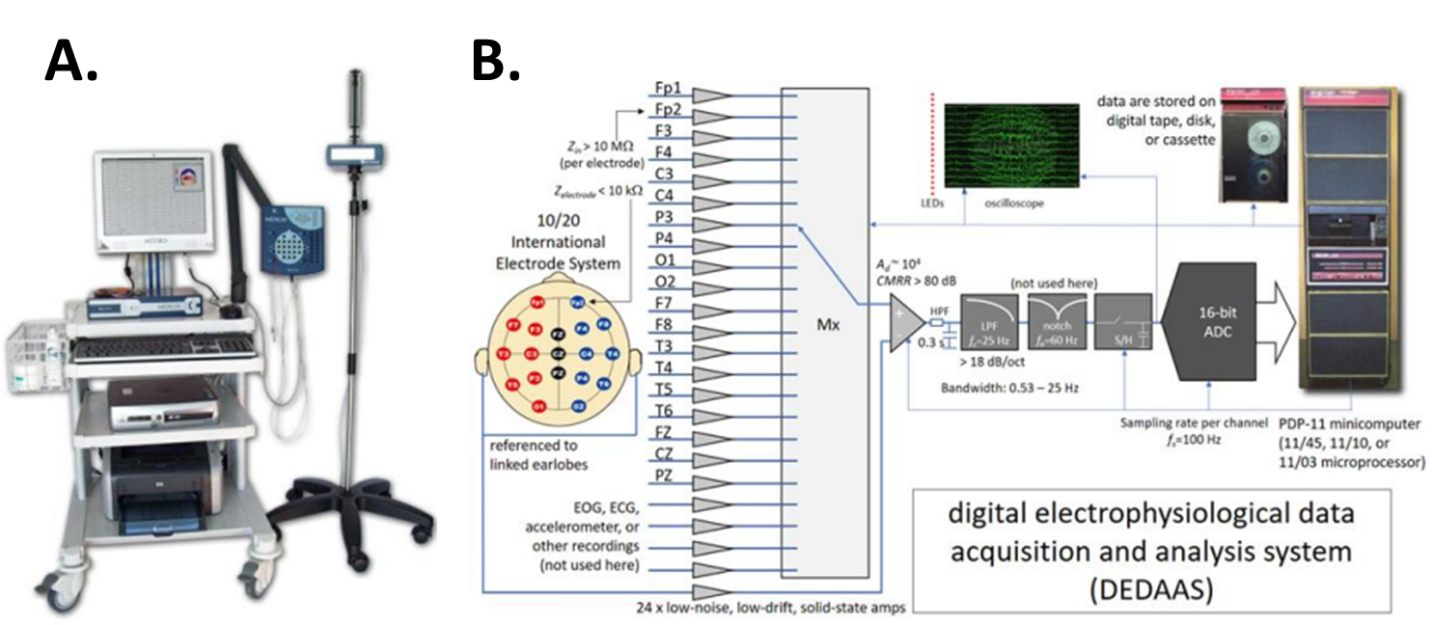
\includegraphics[width=15cm]{pic/Norm/figure3.png}
\caption{不同国家的脑电采集系统。 A.古巴19世纪90年代和2004年左右用的MEDICID 03 Neurometric 系统;B.美国脑电数据采集用的John在19世纪70年代设计的DEDAAS系统;瑞士的脑电数据用的标准Nihon-Kohen系统,暂无图片供显示。}
\label{6:amp}
\end{figure}

\subsection{数据分析方法}\label{6ch:lme}
采用定量脑电技术识别谱特征分为如下步骤:1.电生理专家视觉选出没有明显伪迹且接近稳态过程的数据段;2.因为被试的整体年龄范围较广和个体差异较大难以对每个国家估计相应的头模型,且第二章中发现19通道下零参考与平均参考的效果相当,这里仅将原始脑电数据的连接耳参考变换为平均参考;3.忽略选出脑电记录中可能存在的不连续性,对20多个连续不重叠的2.56s的数据段使用multitaper方法\citing{thomson1982spectrum},设时半带宽积为3.5最大频率为19.14Hz估计交叉谱,得到从0.3906到19.14Hz以0.3906为分辨率的49个频率点。使用谱能量几何均值的方法矫正脑电数据中的全局谱尺度差异\citing{hernandez1994global};4.仅保留交叉谱的对角元,最终每个被试具有931(19电极$\times$49频率)维头表谱特征,不再考虑电极间交叉谱;5.通过视觉甄选多通道脑电功率谱,发现没有出现谱同构的情况; 6.每个被试脑电谱都进行$\log_{10}$转换,目的是进行回归分析时考虑高频谱的作用,如不进行尺度变换高频谱的作用容易被忽略。

为得到与协变量(age、freq、country和individual)有关的谱特征演化曲面,这里采用线性混合效应模型\citing{Demidenko2004,mcculloch2005generalized},该模型在描述因变量与自变量关系时调整多组变量的系数,由线性回归部分的固定效应和与特定区域人群个体相关联的随机效应组成。随机效应可能服从先验分布但固定效应并非如此。线性混合效应模型的标准形式\citing{Demidenko2004}为
\begin{equation*}
\mathbf{y=X\beta+Zb+\epsilon}
\end{equation*}
这里$\mathbf{y}\in{\mathbb{R}^{N_{ef}\times{1}}}$是维度为所有电极$\times$所有频率点的谱值向量,$\mathbf{X}\in{\mathbb{R}^{N_{ef}\times{p}}}$是固定效应设计矩阵,$\mathbf{\beta}\in{\mathbb{R}^{p\times{1}}}$是固定效应的系数向量,$\mathbf{Z}\in{\mathbb{R}^{N_{ef}\times{q}}}$是随机效应设计矩阵,$\mathbf{b}\in{\mathbb{R}^{q\times{1}}}$是随机效应系数向量,$\mathbf{\epsilon}\in{\mathbb{R}^{N_{ef}\times{1}}}$是模型的残差向量。

线性回归模型能检验所有脑电数据的国家和个体因素如何影响$\log_{10}$转换后的功率谱变化。MATLAB内置函数fitlme可以拟合线性混合效应模型,
将相应变量拟合为固定和随机自变量的线性函数。固定效应是5.35-97岁区间内的年龄和0.3906-19.14Hz间的频率;随机效应中国家因素用数字1-4分别表示Cuba 2004、Cuba 1990、Switzerland和United States,所有的个体用数字1-535来表示。尽管Cuba 2004和Cuba 1990来自相同国家,但两次采集的时间间隔很久且被试来自不同地区,因此被假设为具有不同国家因素以增加数据随机性,使构建谱常模中探究国家和个体因素更加严格。

这里通过比较不同模型选出最优线性混合效应模型。用Wilkinson符号\citing{wilkinson1973symbolic}表示三种不同拟合模型,顺次去除一个随机效应:
\bigskip
\begin{description}
	\item[模型一] 固定效应(年龄和频率),随机效应(国家和个体),
	\begin{equation}
	lme_{CI}=\log_{10}(spt)\sim{freq^4\times{age^3}+country+individual}
	\end{equation}
	\item[模型二] 固定效应(年龄和频率),随机效应(国家),
	\begin{equation}
	lme_{C}=\log_{10}(spt)\sim{freq^4\times{age^3}+country}
	\end{equation}
	\item[模型三] 固定效应(年龄和频率),随机效应(空),
	\begin{equation}
	lme=\log_{10}(spt)\sim{freq^4\times{age^3}}
	\end{equation}
\end{description}
\bigskip

因被试数远大于变量数,设计矩阵的奇异性可能影响推断。更复杂的分步线性回归模型可校准从上述三种情况选出的模型找到满足如下两方面的自变量各项系数。即,1.模型中应包含与因变量不太相关的自变量高阶项使模型尽可能完整;2.引入过多自变量高阶项会增大模型复杂度降低预测准确度,要尽可能减少自变量阶数采用更简单模型避免过拟合。采用分步回归能较好地平衡自变量低阶项时的模型简单度和自变量高阶项时的模型复杂度。

另一方法是对$\log_{10}$功率谱采用非参数核回归观察演化曲面如何随年龄和频率变化。采用局部加权的分散平滑方法(locally weighted scatterplot smoothing,LOWESS)\citing{cleveland1979robust,cleveland1988locally,cleveland1981lowess}能结合多个最近邻法基于的子模型,局部利用经典的最小二乘回归,整体通过非线性回归解决用简单方法不能很好解决的问题。这可通过拟合数据的关键自变量得到简单模型,建立能分段描述数据主要变化的函数。其优点在于不需要求出全局函数而是分段拟合数据。

\section{结果}
\subsection{尺度因素去除}
从古巴、瑞士和美国的脑电数据中各随机挑选年龄约20岁的被试并计算功率谱。因为古巴2004左右与19世纪90年代采集的数据尺度相同,这里只显示19世纪90年代的数据。图\ref{6:gsf}A表示不同国家脑电功率谱$\log_{10}$尺度上的幅度存在不同。这种幅度鲜明差异表明功率谱受到尺度因素影响。因此探究国家因素建立定量脑电谱常模演化曲面前必需去除尺度因素。图\ref{6:gsf}B由每个被试原始的$\log_{10}$功率谱减去该被试所有电极$\times$所有频率点下$\log_{10}$谱的平均得到,这种方法就是全局尺度因素去除。图\ref{6:gsf}中三列数据分别来自三个国家约20岁的被试,AB两行是去除尺度因素前后对比,
实际上对所有谱数据都去除了尺度因素。
\begin{figure}[!ht]
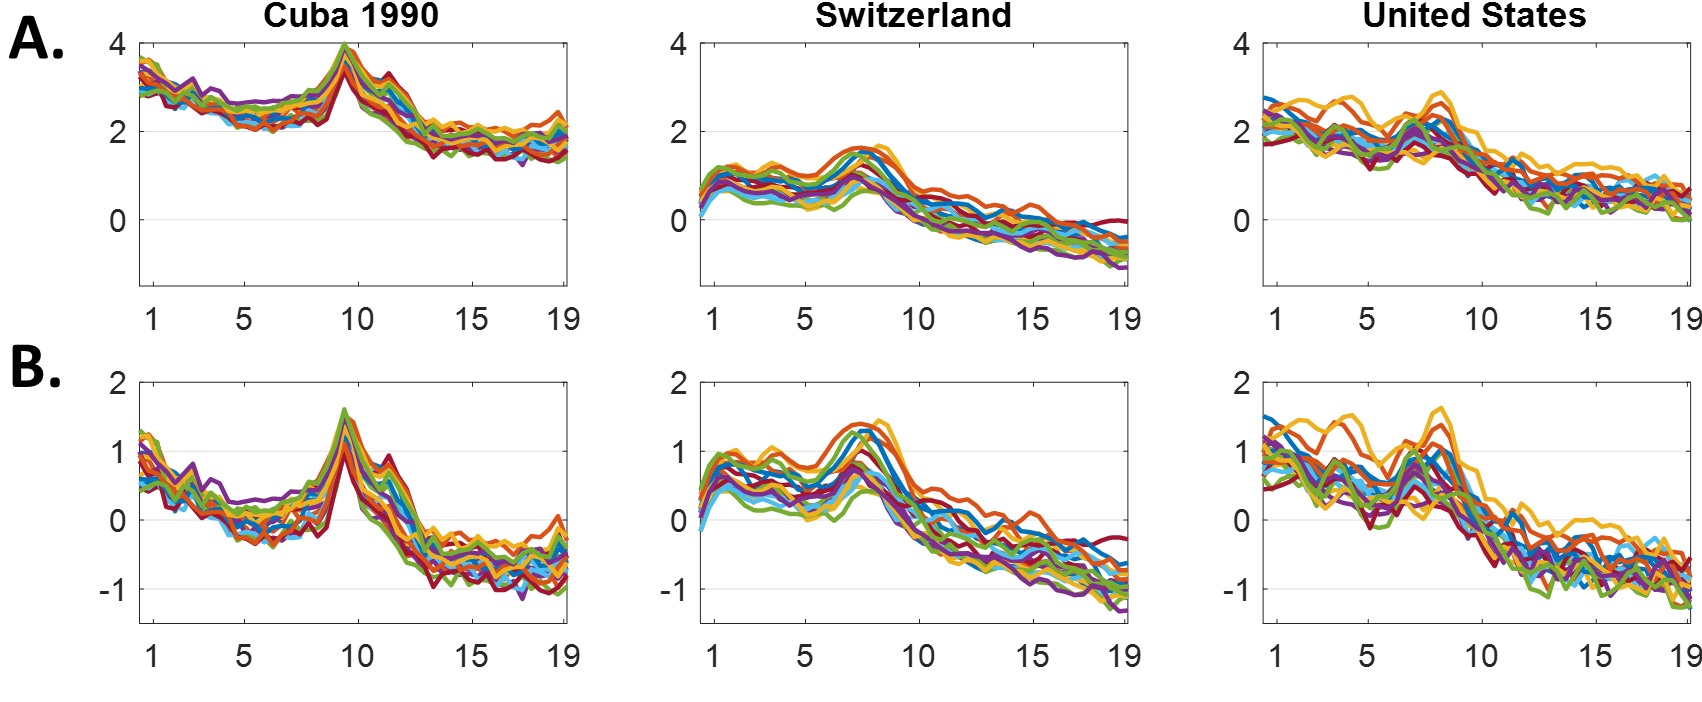
\includegraphics[width=15cm]{pic/Norm/figure4.png}
\caption{谱分析与尺度因素去除。 A.原始尺度; B.去除尺度因素后; 所有子图中,Y轴:$\log_{10}$谱,X轴:0.3906-19.14Hz频率点
,不同颜色曲线代表不同电极位置的谱。}
\label{6:gsf}
\end{figure}

\subsection{混合效应选择}
首先用MATLAB内置函数fitlme拟合\ref{6ch:lme}一节中的三种模型,再用函数compare比较模型二和三,用等式表示为$‘result = compare(lme_{CI}, lme_C, ‘NSim’, ‘1000’)’$和$‘result = compare (lme_C, lme, ‘NSim’, 1000)’$,仿真比较均重复1000次。图\ref{6:pv}表示10-20系统19个电极逐一关于模型间比较的显著性水平,蓝色点表示模型一二$lme_{CI}$与$lme_C$的对比,红色点表示模型二三$lme_C$与$lme$的对比,可以看出所有显著性水平都大于阈值0.05。以电极O1为例,模型一二对比、模型二三对比均不显著,前后二者的显著性水平分别为p=0.062和p=0.50。因此,模型一二和二三的对比依次去除个体和国家这两个对拟合数据不具有显著作用的随机效应,最终保留仅包含固定效应的模型三$\log_{10}(spt)\sim{freq^4\times{age^3}}$作为拟合谱数据的最合理模型。
\begin{figure}[!ht]
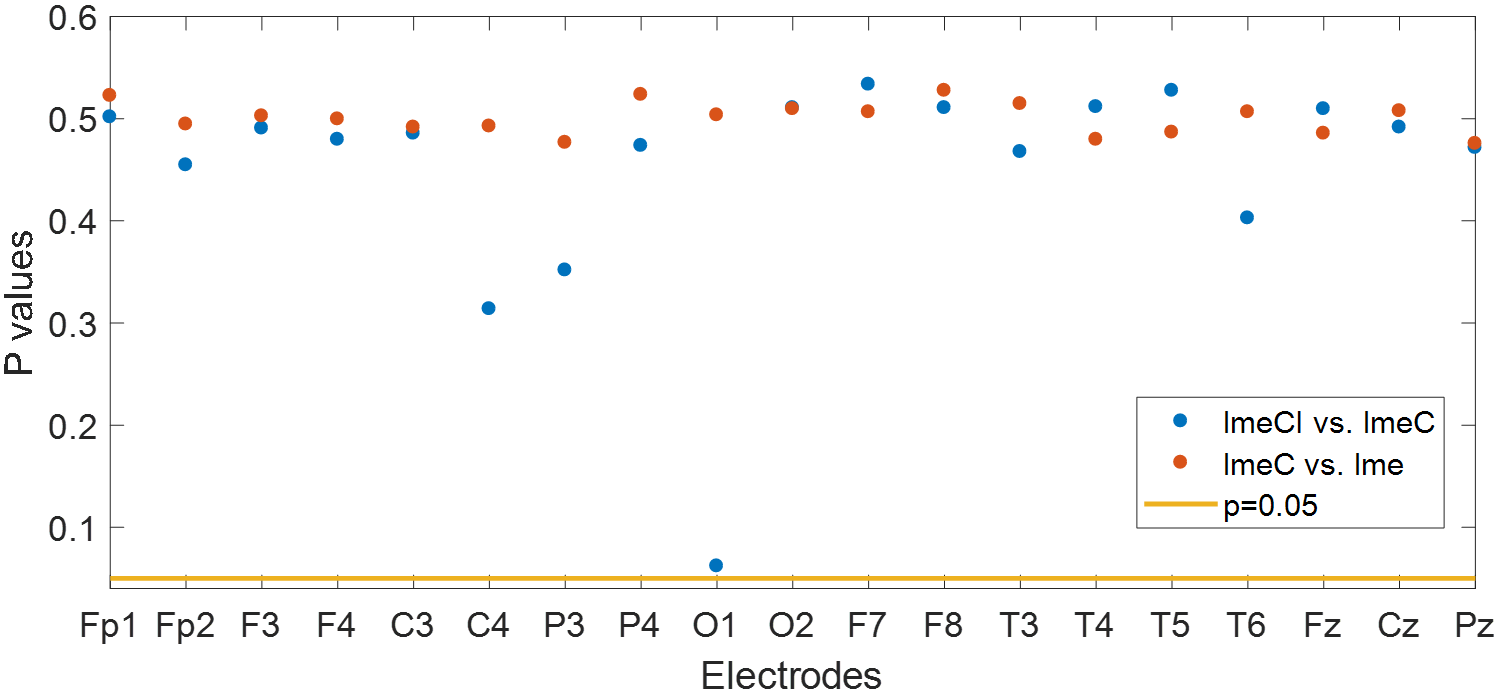
\includegraphics[width=15cm]{pic/Norm/figure5.png}
\caption{使用线性混合效应模型对19个电极逐一进行模型比较的显著性结果。}
\label{6:pv}
\end{figure}

\subsection{分步模型选择}
线性混合效应模型去除了国家和个体因素只保留频率和年龄且二者存在交互作用。进一步使用多项式回归的分步模型选择验证频率与年龄的交互效应。分步模型选择可以估计模型中不同幂次自变量的系数并统计对应幂次项的显著性p值。用MATLAB内置函数stepwiselm假设最高到多项式5次幂的模型$\log_{10}(spt)\sim{freq^5\times{age^5}}$,对所有电极逐一进行模型选择,得到模型系数的tStat和p值。表\ref{6:pvtab}只汇总出电极O1处的结果,表中行和列分别表示频率和年龄不同幂次项并只列出p<0.05的tStat和p值。可以看出频率一次幂对多数年龄项都不显著,频率的高幂次项和年龄的低幂次项因素具有明显交互作用,说明谱随频率的变化比随年龄的变化更复杂,且系数随着多项式的阶数升高而增加,表明数据的复杂度可能被更高阶模型解释。尽管多项式回归可拟合三个国家535例被试在每个电极上功率谱随0.3906-19.14Hz以0.3906为分辨率的49个频率点以及图\ref{6:age}中给定离散年龄值的变化,但被试数535远大于因变量数2造成多项式回归模型的设计矩阵高度奇异,多项式回归模型可能拟合数据中的主要变化但不能进行关于任意频率和任意年龄下功率谱的推断。因此在下一节中采用基于核的非参数回归。
\begin{table}[!h]
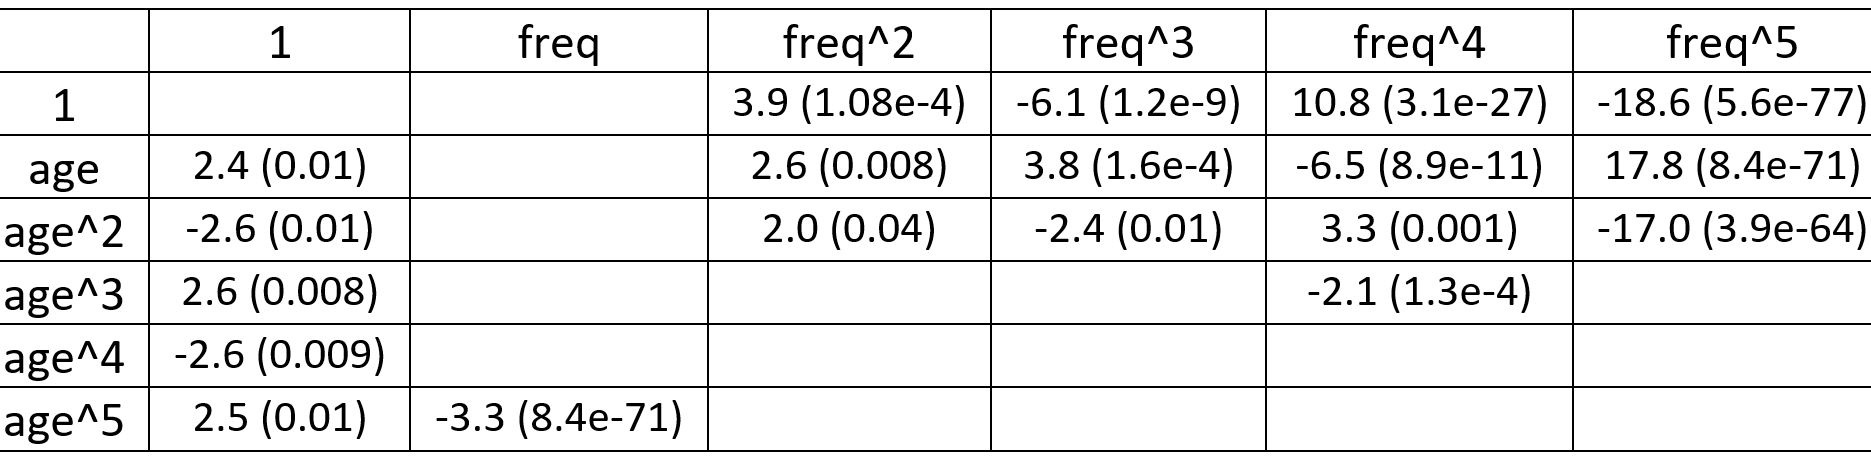
\includegraphics[width=\linewidth]{pic/Norm/pvtab.png}
\caption{电极O1上分步模型多项式回归交互项的tStat值(p值)。p>0.05的交互项略。}
\label{6:pvtab}
\end{table}

\subsection{非参数核回归}
使用LOWESS核回归得到如图\ref{6:surf}中的谱常模演化曲面。图中按照10-20系统的电极相对位置画出每个电极的功率谱随年龄和频率的变化曲面,排在上面的电极(如Fp1、Fp2、F3、F4)指的是头表前额叶区域的电极,左右两侧的电极(如T3、T4)分别对应头表左右颞叶区域的电极,中间和下方的电极(如C3、C4、P3、P4、O1、O2)主要分布在头表顶枕叶区域。所有电极谱曲面颜色具有[-1, 1]的相同尺度,是去除功率谱尺度因素后的共同范围。每个电极上脑电谱随着横轴年龄和纵轴频率的变化曲面就是脑电谱常模演化曲面。观察中间和下方电极上谱的总体演化趋势,发现慢波$\delta$和$\theta$节律在被试年龄较小时快速下降最后随着神经发育成熟明显减弱,$\alpha$节律随着年龄增加直至贯穿整个生命周期逐渐增强。前额叶和顶枕叶区域的电极谱常模演化曲面对比表明低频节律$\delta$、$\theta$在前额叶被试年龄较小时都存在,但$\alpha$节律在儿童和青少年神经发育成熟前逐渐出现并在成年神经发育成熟后明显增强。多数研究表明位于顶枕叶的电极比前额叶的电极更容易记录到$\alpha$节律活动,这一点在谱常模演化曲面上得到体现。大多数电极都表现出慢波$\delta$、$\theta$节律,但位于枕叶的电极(如O1、O2)比额叶的电极(如Fp1、Fp2)呈现衰减更快的趋势,这与多数研究中表明的慢波$\delta$节律主要存在成人前额叶和儿童后枕叶的结果相吻合。

\bigskip
\bigskip
\bigskip
\begin{figure}[!ht]
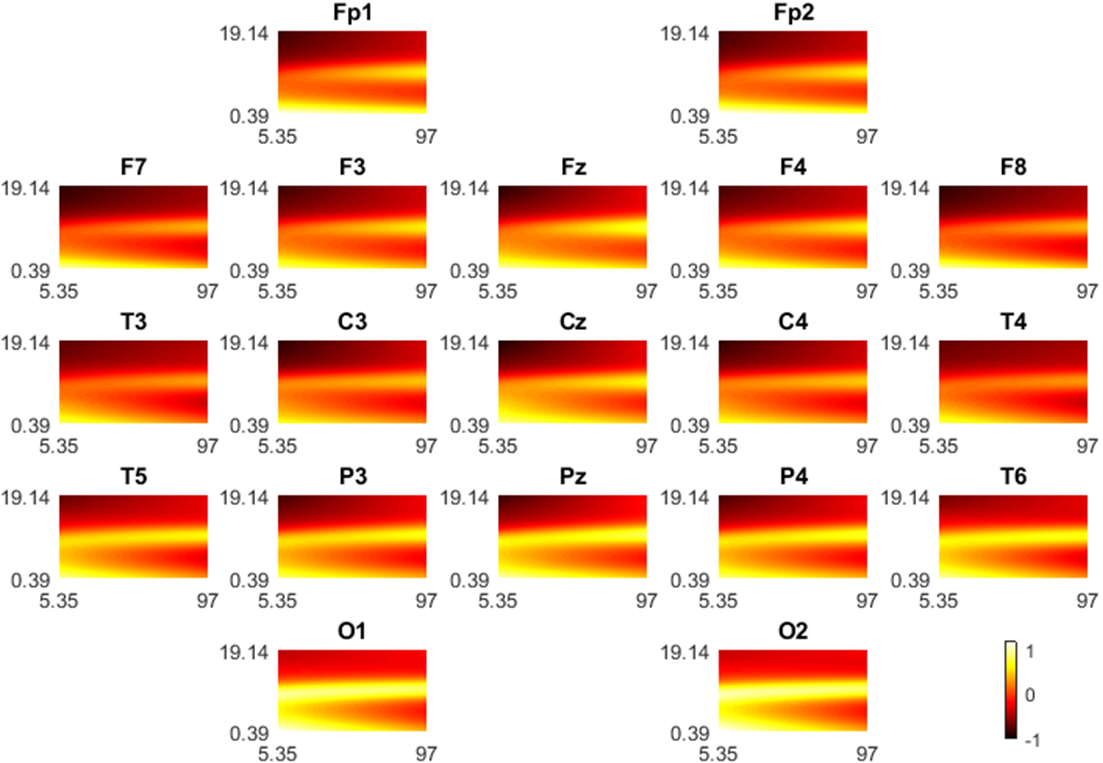
\includegraphics[width=15cm]{pic/Norm/figure6.png}
\caption{脑电谱关于年龄、频率的演化曲面,x轴:5.35 – 97岁,按照$\log_{10}$尺度画出,Y轴: 0.39 – 19.14Hz。}
\label{6:surf}
\end{figure}

\section{讨论}
去除脑电谱因不同采集设备产生的尺度因素,减少尺度对国家、个体因素的影响,采用线性混合效应模型发现国家和个体因素不会对拟合谱数据具有显著影响。这是首次发现被试个体的原始出生国家因素对脑电谱常模演化曲面没有显著影响,肯定建立多国家脑电谱常模的可能性。该结果支持论文\citing{alvarez1987eeg}中直接采用美国人脑电谱常模比较古巴和美国儿童的脑电数据,发现脑电谱常模相对不受社会文化因素影响。本章
肯定出生国家不影响建立反映大脑发育成熟老化过程的谱常模。表\ref{6:pvtab}中总结出电极O1上$\log_{10}$谱与年龄、频率的关系,发现被试年龄和脑电频率具有显著交互效应。这些结果和以前研究\citing{benninger1984eeg,smit2012brain,vandenbosch2019eeg}中的发现高度一致,都发现年龄在个体神经发育中有重要作用。

静息态脑电功率谱一直被认为是与神经发育有关的有效生物标记物。脑电节律与年龄相关呈现不同特点,主要是慢波$\delta$、$\theta$节律谱随年龄增长逐渐衰减和快波$\alpha$、$\beta$节律\citing{ahn1980developmental,john1980developmental,gasser1988development,luchinger2012brain}逐渐增强。论文\citing{lubar1985eeg}发现健康儿童静息态脑电$\theta$节律活动随着$\alpha$节律的明显增强和$\beta$节律的零星出现而变弱。 本章使用非参数回归技术-LOWESS得到对脑电谱演化曲面更详细的描述,凸显神经发育过程中年龄对脑电谱特征的影响。图\ref{6:surf}中所示结果与设想的相同,随着年龄增长慢波$\delta$、$\theta$衰减,$\alpha$波增强,静息态脑电谱显然随着年龄变化。

随年龄增长脑电活动呈现出$\alpha$节律逐渐增加及$\theta$节律逐渐变弱与儿童青少年的神经功能快速发育有关。静息态fMRI和脑电同步采集研究发现儿童发育中的脑电变化主要与年龄有关的神经功能改变有关,静息态BOLD信号的空间相干性可推断出局部和长程脑网络间的整合效应\citing{luchinger2012brain}。本章使用古巴人脑影像计划中覆盖生命周期5.35-97岁的脑电数据综合定量分析儿童神经发育成熟再到个体老化过程中脑电谱特征的变化得到常模演化曲面。尽管论文\citing{szava1994high}已描述覆盖整个生命周期的谱常模演化曲线且采用具有0.3906Hz高频率分辨率的窄带分析,却只分析了古巴19世纪90年代的数据,采用被证明会带有较大失真的连接耳参考以及样条估计,本章采用多国家数据利用平均参考和非参数回归得到的常模演化曲面为定量分析精神紊乱等异常脑电数据提取疾病的脑电生物标记物奠定了基础。

将来需要收集其他国家或社会文化背景更加复杂人群的脑电数据检验这里得到常模的普适性,测试这种常模对疾病诊断中提取生物标记物的敏感性,也可开展脑电溯源分析计算多国家源空间的谱常模,甚至用源空间的脑网络连接指标建立网络连接模式随年龄变化的常模。可能不久基于谱常模和机器学习方法不需要考虑国家或年龄等因素就能预测代表被试神经功能的大脑年龄。
\section{本章小结}
本章分析具有不同社会文化背景的古巴、美国和瑞士脑电数据,采用线性混合效应模型分析发现脑电谱常模不受国家、个体因素的影响,采用非参数回归建立脑电谱常模演化曲面。这是第一个建立多国家通用脑电谱常模的研究。建立的头表脑电谱常模演化曲面覆盖生命周期并具有高频率分辨率,具有局部详细的演化特征。